% RULE APPEARANCE:
\newcommand{\x}{\hspace{1.3pt}} % arithmetic multiplication symbol
\newcommand{\concat}[0]{\bullet}               % list concatenation symbol
\newcommand{\name}[1]{~~\hfill\framebox{#1}}   % for labeling rules

% RULE SPACING:
\newcommand{\skiptop}[0]{\vspace{-13pt}\\}   % for single line on top
\newcommand{\skiptopa}[0]{\vspace{-1pt}\\}   % for first line of two-line top part
\newcommand{\skiptopb}[0]{\vspace{-3pt}\\}   % for second line of two-line top part
\newcommand{\skipbot}[0]{\vspace{-3pt}\\}    % for single line on botto

% HELPER FOR REPEATS:
\newcommand{\tup}[2]{\langle#1, #2\rangle}

% OUR LABEL FOR THE ``POS'' VARIABLE
\newcommand{\pos}[0]{\mbox{\it pos}}

% MY TAB STOP FOR THE PSEUDOCODE
\newcommand{\tab}[0]{\mbox{~~~~}}

%%%%%%%%%%%%%%%%%%%%%%%%%%%%%%%%%%%%%%%%%%%%%%%%%%%%%%%%%%%%%%%%%%%%%%%%%%

\section{Background}

Our transformation requires a specific representation for compressed
data, as well as for programs that transform the data.  The data must
be compressed with LZ77, while the transformation must be expressed in
the cyclo-static dataflow model (e.g., in the StreamIt language).

\subsection{LZ77 Compression}

LZ77 is a lossless, dictionary-based compression algorithm that is
asymptotically optimal~\cite{wyner94optimal}.  LZ77 forms the basis
for many popular compression formats, including ZIP, GZIP and PNG, and
also serves as a generalization of simpler encodings such as Apple
Animation, Microsoft RLE, and Targa.

%% \begin{figure}[t]
%% \begin{minipage}{1.6in}
%% \hspace{-5pt}\begin{tabular}{rcl}
%% stream&\hspace{-9pt}:=&\hspace{-9pt}value$^*$\\ ~ & ~
%% \end{tabular}
%% \end{minipage}
%% \begin{minipage}{1.8in}
%% \hspace{-5pt}\begin{tabular}{rcl}
%% stream&\hspace{-9pt}:=&\hspace{-9pt}(value~$|$~repeat)$^*$ ~ \\
%% repeat&\hspace{-9pt}:=&\hspace{-9pt}$\langle$distance, count$\rangle$
%% \end{tabular}
%% \end{minipage} 
%% ~ \\
%% \begin{minipage}{1.6in}
%% (a) Uncompressed domain
%% \end{minipage}
%% (b) Compressed domain (LZ77)
%% \caption{Representation of data in the uncompressed and compressed
%% domains.  \protect\label{fig:domains}}
%% \end{figure}

The basic idea behind LZ77 is to utilize a sliding window of recently
encoded values as the dictionary for the compression algorithm.  In
the compressed data stream, there are two types of tokens: {\it
  values} and {\it repeats}.  A value indicates a token that should be
copied directly to the output of the decoded stream.  A repeat
$\langle d, c \rangle$ contains two parts: a distance $d$ and a count
$c$.  It indicates that the decoder should start at offset $d$ from
the end of the decoded stream and copy a sequence of $c$ values to the
output.
%The distances are bounded, which enables the decoder to operate with a
%fixed buffer size.  
It is important to note that the count may exceed the distance, in
which case some of the values produced by a repeat operation are also
copied by that operation.  For example, a value A followed by a repeat
$\tup{1}{3}$ results in an output of ``A A A''.  An additional example
is given in Figure~\ref{fig:lz77}.

\begin{figure}[t]
\vspace{-\baselineskip}
\begin{minipage}{3in}
\mbox{~}
\begin{center}
\psfig{figure=lz77-figure.eps,width=3in}
\caption{Example of LZ77 decompression.
\protect\label{fig:lz77}}
\end{center}
\end{minipage}
\hspace{0.25in}
\begin{minipage}{2.65in}
\mbox{~}\hspace{0.5in}\psfig{figure=streamit-figure.eps,width=1.5in}
\vspace{4pt}
\caption{Example stream graph in which pixels are interleaved by a
  joiner and then combined using a matte.  Edges are annotated with
  the I/O rates.\protect\label{fig:streamit}}
\end{minipage}
\vspace{-\baselineskip}
\end{figure}

\subsection{Cyclo-Static Dataflow}

The basic idea behind cyclo-static
dataflow~\cite{bilsen95-cyclostatic,LM87-i} is to represent a program
as a block diagram, in which independent components (called {\it
  actors}) communicate over FIFO data channels (see
Figure~\ref{fig:streamit}).  One can think of an actor as a function
(called repeatedly by the runtime system) that consumes items from the
input tapes and produces items on the output tapes.  Actors must
declare how many items they will produce and consume on each
execution; these I/O rates must either be constant across all
executions, or must follow a fixed cycle.  In this paper, actors may
not retain internal state between executions.

We use the StreamIt language~\cite{streamitcc} to express cyclo-static
dataflow programs.  There are three kinds of actors in StreamIt, and
our analysis handles each one separately:
\begin{itemize}

\item \vspace{-2mm} {\bf Filters} have a single input stream and a
  single output stream, and perform general-purpose computations as
  specified by the programmer.

\item \vspace{-2mm} {\bf Joiners} interleave multiple input streams into a single
  output stream.  Items are interleaved in a roundrobin pattern
  according to a set of {\it weights}; for example, weights of $(n_1,
  n_2)$ indicate that the first $n_1$ items are drawn from the first
  input stream, and the next $n_2$ items are drawn from the second
  input stream.

\item \vspace{-2mm} {\bf Splitters} have a single input stream and multiple output
  streams.  They may perform either roundrobin distribution, or
  duplicate distribution. \vspace{-2mm}

\end{itemize}

\section{Mapping into the Compressed Domain}

Our technique allows any cyclo-static dataflow program to operate
directly on LZ77-compressed data.  Rather than modifying the code
within the actors, our transformation treats actors as black boxes and
wraps them in a new execution layer.  The transformation attempts to
preserve as much compression as possible without ever performing an
explicit re-compression step.  While there exist cases in which the
output data will not be as compressed as possible, under certain
conditions the output is guaranteed to be fully compressed (relative
to the compression of the input).  We quantify this issue later.

To describe the mapping into the compressed domain, we consider each
StreamIt construct in turn.  Filters and joiners are described below,
while (due to space limitations) splitters are described in our
companion technical report~\cite{techreport}.

\subsection{Filters}

The procedure for translating a filter into the compressed domain is
given in Figure~\ref{fig:translate}(a), and an example appears in
Figure~\ref{fig:filter-example}.  The behavior of the
compressed-domain filter can be considered in two pieces.  The first
piece consists of the simple case (annotated {\it pass-uncompressed}
in the code) in which the upcoming inputs to the filter are
uncompressed values.  In this case, the original filter is called with
those inputs, transforming $n$ input items to $m$ output items.  The
rest of the code deals with repeat tokens, attempting to translate
them across the filter with the minimum decompression needed.

The {\bf key idea of the paper} is encapsulated in the {\it
  pass-compressed} case in Figure~\ref{fig:translate}(a).  This rule
specifies how to translate a repeat token directly from a filter's
input tape to a filter's output tape without invoking the filter's
computation.  This translation is possible whenever the repeat
distance $d$ is a multiple of the filter's input rate $n$.  In other
words, the repeat is aligned with the execution boundaries of the
actor, so invoking the actor would produce the same results as before.
In transferring the repeat token to the output tape, two adjustments
are made: 1) the distance and count are scaled by a factor of $m/n$ to
reflect possible differences between the output ($m$) and input ($n$)
rates of the actor, and 2) if the count is not an even multiple of the
input rate, then some leftover items ($c\%n$, where $\%$ represents
the modulo operation) are left on the input tape.

In cases where the repeat distance does not match the granularity of
the actor, the distance can sometimes be adjusted to allow
compressed-domain processing.  The {\it coarsen-repeat} rule
represents such an adjustment.  Consider that a filter inputs two
items at a time, but encounters a long repeat with distance three and
count 100.  That is, the input stream contains a regular pattern of
values with periodicity three.  Though consecutive executions of the
filter are aligned at different offsets in this pattern, every third
filter execution (spanning six values) falls at the same alignment.
In general, a repeat with distance $d$ can be exploited by a filter
with input rate $n$ by expanding the distance to $\mbox{LCM}(d, n)$.
In order to perform this expansion, the count must be greater than the
distance, as otherwise the repeat references old data that may have no
periodicity.  Also, the stream needs to be padded with $\mbox{LCM}-d$
values before the coarsened repeat can begin; this padding takes the
form of a shorter repeat using the original distance.

A second way to adjust a repeat token for compressed-domain processing
is by changing its count rather than its distance (rule {\it expand}).
The expand rule is invoked if a repeat has a count less than $n$, if
it is unaligned with the boundaries of an actor's execution, or if its
distance is not a multiple of $n$ (and cannot be coarsened
appropriately).  The expand rule decodes a single value from a repeat
token, thereby decreasing its count by one; the rest of the repeat may
become aligned later.  If the count of a repeat reaches zero, it is
eliminated.

Note that the {\it expand} rule requires partial decompression of the
data stream.  In order to perform this decompression, it may be
necessary to maintain an auxiliary data structure--separate from the
filter's input stream--that holds a complete window of decompressed
data.  This auxiliary structure is needed because the sliding-window
dictionary of LZ77 makes it difficult to decode one element without
decoding others.  However, even if the stream is fully decompressed in
parallel with the main computation, our technique retains many
benefits because the filters still operate on the compressed stream;
the volume of data processed is reduced, and the cost of
re-compression is averted.  For general algorithms such as gzip,
compression can be up to 10x slower than
decompression~\cite{ziviani00compression}.

%% The alignment stage sometimes needs to partially decompress the
%% data in the stream.  Due to the sliding-window dictionary in LZ77,
%% in general it is difficult to decode only a few items without
%% decompressing others.  Thus, our formulation assumes that a fully
%% decompressed version of the stream is available; the transition
%% rules access the decompressed data using the \mbox{\it decode}
%% function, which returns the sequence of values represented by a
%% repeat token at its current position in the stream.  However, in
%% practice, this decompression can be avoided whenever the repeat
%% distance is the same as the window size, as this simply causes a
%% value in the window to be overwritten by itself.  This case is very
%% common in several practical compression formats; for example, in
%% Apple Animation, the vast majority of repeats reference the same
%% pixel in the previous frame (which is also the window size), and
%% thus most decompression is avoided.  In run-length encoding, the
%% repeat distance and the window size are always equal to one, so no
%% decompression is needed.  While general LZ77 does require a
%% decompressed window to be maintained, our technique still offers
%% significant benefits by computing on a smaller volume of data and
%% avoiding the cost of re-compression.  For general algorithms such
%% as gzip, compression can be up to 10x slower than
%% decompression~\cite{ziviani00compression}.

\newcommand{\mynewline}[0]{\\ \vspace{-1pt}}
\begin{figure}[t]
\vspace{-0.4\baselineskip}
\hspace{-33pt}
\begin{minipage}{0.53\textwidth}
\begin{small}
{\it Execute a filter in the compressed domain, given that it consumes
  $n$ items and produces $m$ items on each execution.}\mynewline
\textsc{Execute-Compressed-Filter}~(int $n$, int $m$) \{\mynewline
\mbox{~~~~}{\bf while true} \{\mynewline
\mbox{~~~~}\mbox{~~~~}{\it /* pass-uncompressed */} \mynewline
\mbox{~~~~}\mbox{~~~~}{\bf if} input {\bf endswith} $n$ values {\bf then}\mynewline
\mbox{~~~~}\mbox{~~~~}\mbox{~~~~}{\bf execute} one call to uncompressed filter\mynewline
\mbox{~~~~}\mbox{~~~~}~\mynewline
\mbox{~~~~}\mbox{~~~~}{\it /* pass-compressed */} \mynewline
\mbox{~~~~}\mbox{~~~~}{\bf else if} input {\bf endswith} $\langle d,c \rangle$\mynewline
\mbox{~~~~}\mbox{~~~~}\mbox{~~~~~~~}{\bf and} $d\%n = 0$ {\bf and} $c \geq n$ {\bf then}\mynewline
\mbox{~~~~}\mbox{~~~~}\mbox{~~~~}{\bf replace} $\langle d,c \rangle$ with $\langle d, c\%n\rangle$ on input\mynewline
\mbox{~~~~}\mbox{~~~~}\mbox{~~~~}{\bf push} $\langle m~d/n, m~(c-c\%n)/n \rangle$ to output\mynewline
\mbox{~~~~}\mbox{~~~~}~\mynewline
\mbox{~~~~}\mbox{~~~~}{\bf else}\mynewline
\mbox{~~~~}\mbox{~~~~}\mbox{~~~~}{\bf let} $\langle d,c \rangle = $ last repeat on input\mynewline
\mbox{~~~~}\mbox{~~~~}\mynewline
\mbox{~~~~}\mbox{~~~~}\mbox{~~~~}{\it /* coarsen-repeat */}\mynewline
\mbox{~~~~}\mbox{~~~~}\mbox{~~~~}{\bf let} $L = \mbox{LCM}(d, n)$\mynewline
\mbox{~~~~}\mbox{~~~~}\mbox{~~~~}{\bf if} $d < L < c$ {\bf then} {\bf replace} $\langle d,c \rangle$\mynewline
\mbox{~~~~}\mbox{~~~~}\mbox{~~~~}\mbox{~~~~}\mbox{~~~~~}with $\langle c - (L - d) \rangle, \langle d, L - d\rangle$ on input\mynewline
\mbox{~~~~}\mbox{~~~~}\mynewline
\mbox{~~~~}\mbox{~~~~}\mbox{~~~~}{\it /* expand */}\mynewline
\mbox{~~~~}\mbox{~~~~}\mbox{~~~~}{\bf else if} $c > 0$ {\bf then}\mynewline
\mbox{~~~~}\mbox{~~~~}\mbox{~~~~}\mbox{~~~~}{\bf decode} $\langle d,c \rangle$ into $\langle d,c-1\rangle,V$ on input\mynewline
\mbox{~~~~}\mbox{~~~~}\mbox{~~~~}{\bf else}\mynewline
\mbox{~~~~}\mbox{~~~~}\mbox{~~~~}\mbox{~~~~}{\bf remove} $\langle d,c \rangle$ from input\mynewline
\mbox{~~~~}\}\mynewline
\}~~~~~~~~~~~~~~~~~~~~~~~~~~~~~~~~~~~~~~~~~~~~~~{\bf (a)}\mynewline
\end{small}
\end{minipage}
\hspace{0.2in}
\begin{minipage}{0.59\textwidth}
\begin{small}
{\it Execute a roundrobin joiner in the compressed domain, given that
  it inputs $n_1$ items from input1 and $n_2$ items from input2 on
  each execution.}\mynewline
\textsc{Execute-Compressed-Joiner}~(int $n_1$, int $n_2$) \{\mynewline
\mbox{~~~~}{\bf while true} \{\mynewline \mbox{~~~~}\mbox{~~~~}{\it /*
  pass-uncompressed */}\mynewline \mbox{~~~~}\mbox{~~~~}{\bf if}
input1 {\bf endswith} value\mynewline
\mbox{~~~~}\mbox{~~~~}\mbox{~~~~}{\bf transfer} value from input1 to
output\mynewline \mbox{~~~~}\mbox{~~~~}\mynewline
\mbox{~~~~}\mbox{~~~~}{\it /* pass-compressed-long */}\mynewline
\mbox{~~~~}\mbox{~~~~}{\bf else if} input1 {\bf endswith} $\langle
d_1,c_1 \rangle$ {\bf and} $d_1\%n_1 = 0$\mynewline
\mbox{~~~~}\mbox{~~~~}\mbox{~~~~~~~}{\bf and} input2 {\bf endswith}
$\langle d_2,c_2 \rangle$ {\bf and} $d_2\%n_2 = 0$\mynewline
\mbox{~~~~}\mbox{~~~~}\mbox{~~~~~~~}{\bf and} $d_1/n_1 = d_2/n_2$ {\bf
  then}\mynewline \mbox{~~~~}\mbox{~~~~}\mbox{~~~~}{\bf let} $(L_1,
L_2)$ = \textsc{Repeat\_Lengths}($c_1$, $c_2$, {\it pos})\mynewline
\mbox{~~~~}\mbox{~~~~}\mbox{~~~~}{\bf replace} $\langle d_1, c_1
\rangle$ with $\langle d_1, c_1-L_1\rangle$ on input1\mynewline
\mbox{~~~~}\mbox{~~~~}\mbox{~~~~}{\bf replace} $\langle d_1, c_2
\rangle$ with $\langle d_2, c_2-L_2\rangle$ on input2\mynewline
\mbox{~~~~}\mbox{~~~~}\mbox{~~~~}{\bf push} $\langle d_1(n_1+n_2)/n_1,
L_1+L_2 \rangle$ to output\mynewline \mbox{~~~~}\mbox{~~~~}\mynewline
\mbox{~~~~}\mbox{~~~~}{\it /* pass-compressed-short */}\mynewline
\mbox{~~~~}\mbox{~~~~}{\bf else if} input1 {\bf endswith} $\langle
d_1,c_1 \rangle$ {\bf and} $c_1>0$\mynewline
\mbox{~~~~}\mbox{~~~~}\mbox{~~~~}{\bf let} offset = {\bf if} $d\%n_1
\leq \mbox{\it pos}$ {\bf then} {\it pos} {\bf else} $d\%n_1 +
n_2$\mynewline \mbox{~~~~}\mbox{~~~~}\mbox{~~~~}{\bf let} L = {\bf
  min}($c$, \textsc{Join\_Potential}($d$))\mynewline
\mbox{~~~~}\mbox{~~~~}\mbox{~~~~}{\bf replace} $\langle d, c\rangle$
with $\langle d, c - L\rangle$ on input1\mynewline
\mbox{~~~~}\mbox{~~~~}\mbox{~~~~}{\bf push} $\langle
(n_1+n_2)~\mbox{\bf floor}(d/n_1) + \mbox{offset}, L \rangle$ to
output\mynewline \mbox{~~~~}\mbox{~~~~}\mynewline
\mbox{~~~~}\mbox{~~~~}{\it /* prune */}\mynewline
\mbox{~~~~}\mbox{~~~~}{\bf else~} {\it /* input1 endswith}~$\langle
d_1, 0 \rangle$~{\it */}\mynewline
\mbox{~~~~}\mbox{~~~~}\mbox{~~~~}{\bf remove} $\langle d_1,0 \rangle$
from input1\mynewline \mbox{~~~~}\}\mynewline
\}~~~~~~~~~~~~~~~~~~~~~~~~~~~~~~~~~~~~{\bf (b)}\mynewline
\end{small}
\end{minipage}
\vspace{-1.5\baselineskip}
\caption{Translation of (a) filters and (b) joiners into the
  compressed domain.  We use $\%$ to denote a modulo operation.
%Helper functions appear in Figure~\ref{fig:helpers}.
\protect\label{fig:translate}}
\vspace{-4pt}
\end{figure}

\subsection{Joiners}

%% It is necessary to consider splitters and joiners separately from
%% general-purpose actors because of their pass-through semantics: the
%% inputs are distributed to the outputs without performing any
%% computation.  Our translation to the compressed domain leverages this
%% fact to preserve considerably more compression than would be possible
%% if splitters and joiners were viewed as opaque computational nodes
%% with multiple inputs and multiple outputs.

The procedure for executing a joiner in the compressed domain appears
in Figure~\ref{fig:translate}(b), while an example appears in
Figure~\ref{fig:sj-example}.  To simplify the presentation, we
consider a joiner with only two input streams.  This captures all of
the fundamental ideas; extension to additional streams is
straightforward.  In addition, we use the following notations:

\begin{figure*}[t]
\hspace{-0.04\textwidth}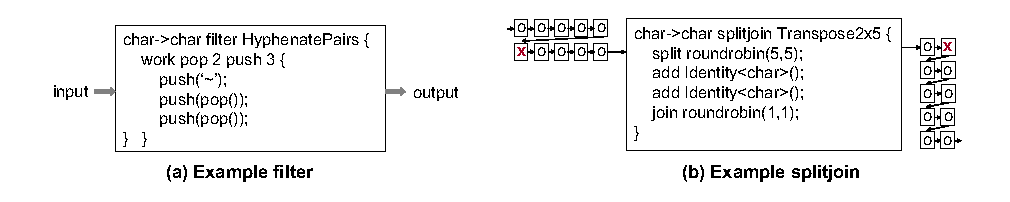
\psfig{file=compressed-filters-in-streamit.eps,width=1.08\textwidth}

\vspace{-10pt}
\caption{Example filter, splitter, and joiner in StreamIt.  The
  splitter and joiner combine to form a Transpose. Translation to the
  compressed domain is illustrated in Figures~\ref{fig:filter-example}
  and~\ref{fig:sj-example}.\protect\label{fig:streamit-example}}
\vspace{1pt}
\end{figure*}

\begin{figure*}[t]
\hspace{-0.045\textwidth}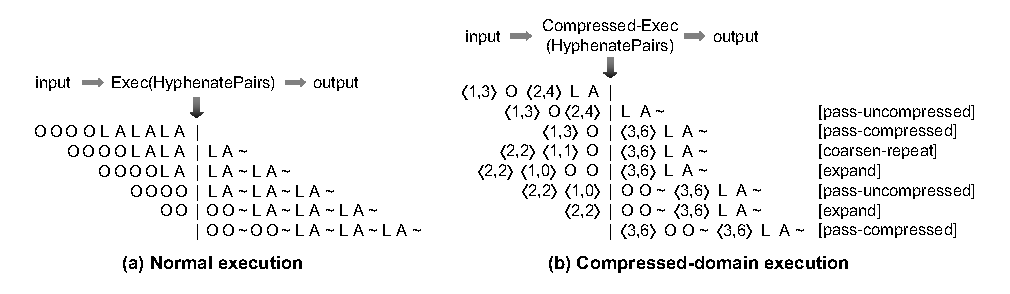
\psfig{file=compressed-filter-example.eps,width=1.09\textwidth}

\vspace{-10pt}
\caption{Example execution of a filter in the uncompressed and
  compressed domains.  See Figure~\ref{fig:streamit-example}(a) for the
  source filter.\protect\label{fig:filter-example}}
\vspace{-6pt}
\end{figure*}

\begin{figure*}[t]
\hspace{-0.045\textwidth}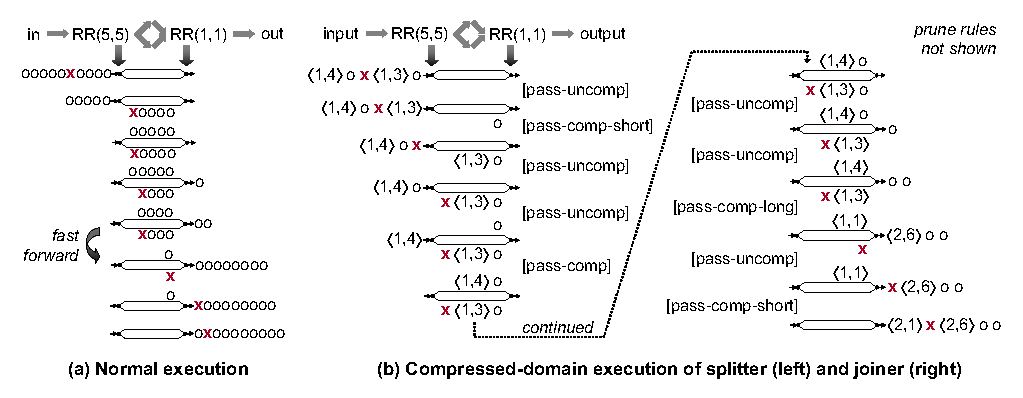
\psfig{file=compressed-splitjoin-example.eps,width=1.09\textwidth}

\vspace{-10pt}
\caption{Example execution of splitters and joiners in the compressed
  domain.  As illustrated by the input/output pairs in
  Figure~\ref{fig:streamit-example}(b), the example performs a transpose
  of a 2x5 matrix.  When the matrix is linearized as shown here, the
  input stream traverses the elements row-wise while the output stream
  traverses column-wise.  Due to redundancy in the matrix, this
  reordering can be done largely in the compressed domain.
  \protect\label{fig:sj-example}}
\vspace{-3pt}
\end{figure*}

\begin{itemize}

\item \vspace{-2mm} As mentioned previously, splitters and joiners
  adopt a fine-grained cyclo-static execution model, in which each
  execution step transfers only one item from an input tape to an
  output tape.  That is, a roundrobin$(n_1, n_2)$ joiner has $n_1 +
  n_2$ distinct execution steps.  We refer to every group of $n_1 +
  n_2$ steps as an {\it execution cycle}.

\item \vspace{-2mm} The pseudocode in Figure~\ref{fig:translate}
  assumes, without loss of generality, that the next execution step of
  the joiner will read from the first input stream (input1).

\item \vspace{-2mm} We use $\pos$ to denote the number of items (in
  terms of the uncompressed domain) that have already been read from
  the current input stream (input1) in the current execution cycle.
  For brevity, the pseudocode does not maintain the value of $\pos$,
  though it is straightforward to do so.\vspace{-2mm}

\end{itemize}

There are two ways to pass repeat tokens through a joiner.  If the
input streams contain compatible repeat tokens, then they can be
combined into a long repeat that spans multiple execution cycles;
otherwise, a shorter repeat is extracted from only one of the streams.

The first and most powerful way to execute joiners in the compressed
domain is to combine repeat tokens from both input streams (case {\it
  pass-compressed-long} in Figure~\ref{fig:translate}b).  For this to
be possible, both repeat distances must be the same multiple of their
respective joiner weight ($n_1$ or $n_2$); the combined token has a
repeat distance that is a multiple of $n_1 + n_2$.  The
\textsc{Repeat\_Length} routine (detailed in our technical
report~\cite{techreport}) calculates the maximum repeat length
depending on the current position of the joiner and the repeat lengths
of the inputs.

The second mode of compressed joiner execution ({\it
  pass-compressed-short}) inputs only a single repeat token,
extracting the maximum length that can safely move to the output.  The
\textsc{Join\_Potential} routine (detailed in our technical
report~\cite{techreport}) determines how much of the repeat can be
moved to the output before the data referenced would have originated
from a different input stream.

%% \begin{figure}[t]
%% \small
%% \textsc{run\_joiner}$(c_1, c_2, \pos )${\it ~returns the number of
%%   items that can be read from each input stream before one of them is
%%   exhausted.  Assumes that $c_1$ and $c_2$ items are available on the
%%   first and second input streams, and that the joiner starts by
%%   reading from position \mbox{pos} of the first input stream.}
%% ~ \\ ~ \\
%% %Assumes that only a
%% %  single repeat token is available (i.e., the {\tt
%% %    pass-compressed-long} rule does not apply).} ~ \\
%% \textsc{Join\_Potential}$(d)${\it ~returns the maximum count of a
%%   repeat token that could safely be emitted to the output stream,
%%   given that ther is a repeat token with distance $d$ on the current
%%   input.}
%% \caption{Helper functions for translating joiners into the compressed
%%   domain.  For implementation details, see our technical
%%   report~\cite{techreport}.  \protect\label{fig:helpers}}
%% \end{figure}

%% \newcommand{\tablesep}{\hspace{-3.5pt}}
%% \begin{figure}[t]
%% \hspace{-5pt}\begin{tabular}{llll}
%% \multicolumn{2}{l}{Variables} & \multicolumn{2}{l}{{\tablesep}Constants} \\ \rule[10pt]{1.9in}{0.3pt}\hspace{0.1in}\rule[10pt]{1.3in}{0.3pt}\hspace{-1.3in}\hspace{-2pt}\hspace{-1.97in}\hspace{-2pt}
%% $S$, $T$ & {\tablesep}Input, output streams & {\tablesep}$n_1$, $n_2$ & {\tablesep}Actor's pop rates \\
%% $V$ & {\tablesep}List of values (may be empty) & {\tablesep}$m$ & {\tablesep}Actor's push rate \\
%% $\tup{d}{c}$ & {\tablesep}Repeat distance \& count & {\tablesep}~ & ~ \vspace{6pt} \\
%% \multicolumn{2}{l}{Functions (list $\times$ list $\rightarrow$ list)}& ~ & ~ \\ \rule[10pt]{3.3in}{0.3pt}\hspace{-3.3in}
%% $\concat$ & {\tablesep}List concatenation & ~ & ~ \\
%% $F$ & \multicolumn{3}{l}{{\tablesep}Filter work function, outputs $m$-element list}
%% \end{tabular}
%% \caption{Notations used in the semantic rules.\protect\label{fig:notations}}
%% \end{figure}

%% \begin{figure}[t]
%% $S \concat V \rightarrow T~~~~|V|=n$\name{exec-uncompressed} \skiptopb
%% ---------------------------- \skipbot
%% $S \rightarrow F(V) \concat T$
%% \caption{Semantics of \textsc{Exec(F)}: execution of filter F in the
%% uncompressed domain.  Notations are defined in Figure~\ref{fig:notations}.
%% \protect\label{fig:exec-rule}}
%% \end{figure}

%% \begin{figure}[t]
%% ~~~~~~~~~\psfig{figure=actor-figure.eps,width=2.8in}

%% \mbox{~}(a) Uncompressed domain~~~~~~~~~~~~~~~~~(b) Compressed domain
%% \caption{Overall execution of a filter F in the uncompressed and compressed domains.
%% \protect\label{fig:actor-pic}}
%% \end{figure}

%% Filter execution in the uncompressed domain is described by the rule
%% in Figure~\ref{fig:exec-rule}.  The rule expresses the simple fact
%% that a filter inputs a list of $n$ values from the end of its input
%% stream; this list is denoted by $V$.  The filter pushes its results,
%% denoted by $F(V)$, onto the front of the output stream.

%% \begin{figure*}[t]
%% \vspace{-6pt}
%% \hspace{-0.5in}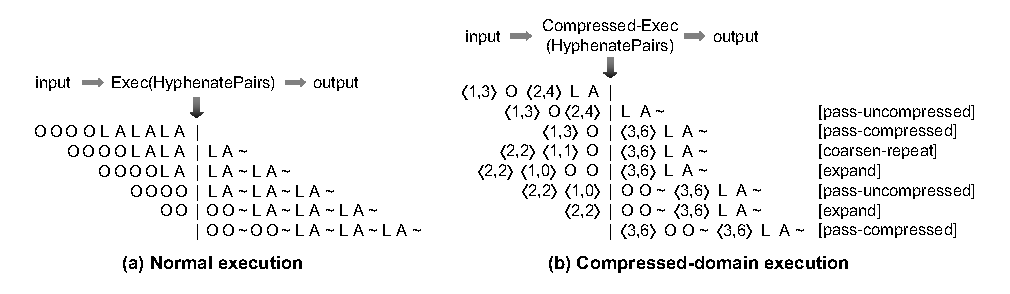
\psfig{file=compressed-filter-example.eps,width=7in}
%% \vspace{6pt}
%% \caption{Example execution of a filter in the uncompressed and
%%   compressed domains.\protect\label{fig:filter-example}}
%% \end{figure*}

%% \begin{figure}[t]
%% $S \concat V \rightarrow T~~~~|V|=n$\name{exec-uncompressed} \skiptopb
%% ---------------------------- \skipbot
%% $S \rightarrow F(V) \concat T$
%% ~ \\ ~ \\
%% %\hfill\mbox{\it Same as above.}\name{exec-uncompressed}\vspace{6pt}\\
%% $S \concat \tup{d}{c} \rightarrow T~~~~d$\%$n=0~~~~c$\%$n=0$\name{exec-compressed} \skiptopb
%% ------------------------------------------------ \skipbot
%% $S \rightarrow \tup{m{\x}d/n}{m{\x}c/n} \concat T$
%% \caption{Semantics of \textsc{Compressed-Exec(F)}: execution of filter
%% $F$ in the compressed domain.
%% %This filter also includes an {\tt exec-uncompressed} rule, which is
%% %identical to the one in Figure~\ref{fig:exec-rule}.
%% Notations are defined in Figure~\ref{fig:notations}.
%% \protect\label{fig:compressed-exec-rule}}
%% \end{figure}

%% Filter execution in the compressed domain requires a two-stage
%% transformation (see Figure~\ref{fig:actor-pic} for an overview, and
%% Figure~\ref{fig:filter-example} for a detailed example).  First, the
%% input stream is aligned to a granularity $n$ that matches the input
%% rate of the filter.  This alignment guarantees that every token in the
%% stream is either a sequence of $n$ values, or a repeat in which both
%% the distance and the count are multiples of $n$.  The alignment stage
%% (described in detail later) is a no-op for filters that pop only one
%% item ($n=1$).

%% After the alignment stage comes the execution of the compressed
%% filter, which appears in Figure~\ref{fig:compressed-exec-rule}.  The
%% {\tt exec-uncompressed} rule
%% %(not shown in Figure~\ref{fig:compressed-exec-rule}) 
%% deals with values on the input stream, and is identical to that in the
%% uncompressed execution.  The {\tt exec-compressed} rule deals with
%% repeats on the input stream and encapsulates the key idea of the
%% paper.  Because the inputs are repeating at the correct granularity,
%% the repeat can be copied directly to the output of the filter without
%% performing any new computation.  The only change needed is to adjust
%% the repeat distance and count to match the filter's output rate.

%% \subsubsection{Stream Alignment}

%% The alignment phase is needed for filters that pop more than one item
%% from the input stream.  Its goal is to align the execution boundaries
%% of the filter with the repeat boundaries of the compressed data; this
%% alignment is required for the compressed execution.  Following
%% alignment, each execution of a filter will input either $n$
%% consecutive values, or a repeat token with a distance and count that
%% are evenly divisible by $n$ (where $n$ represents the pop rate of the
%% filter).

%% The alignment stage sometimes needs to partially decompress the data
%% in the stream.  Due to the sliding-window dictionary in LZ77, in
%% general it is difficult to decode only a few items without
%% decompressing others.  Thus, our formulation assumes that a fully
%% decompressed version of the stream is available; the transition rules
%% access the decompressed data using the \mbox{\it decode} function,
%% which returns the sequence of values represented by a repeat token at
%% its current position in the stream.  However, in practice, this
%% decompression can be avoided whenever the repeat distance is the same
%% as the window size, as this simply causes a value in the window to be
%% overwritten by itself.  This case is very common in several practical
%% compression formats; for example, in Apple Animation, the vast
%% majority of repeats reference the same pixel in the previous frame
%% (which is also the window size), and thus most decompression is
%% avoided.  In run-length encoding, the repeat distance and the window
%% size are always equal to one, so no decompression is needed.  While
%% general LZ77 does require a decompressed window to be maintained, our
%% technique still offers significant benefits by computing on a smaller
%% volume of data and avoiding the cost of re-compression.  For general
%% algorithms such as gzip, compression can be up to 10x slower than
%% decompression~\cite{ziviani00compression}.

%% The semantics of stream alignment are given in
%% Figure~\ref{fig:stream-align}.  If the end of the input stream
%% contains $n$ values, then alignment is satisfied and the values are
%% moved to the output stream (rule {\tt pass-uncompressed}).  Likewise,
%% if the input contains a repeat in which the distance is a multiple of
%% $n$ and the count is at least $n$, then a number of aligned repeats
%% are peeled from the input and moved to the output (rule {\tt
%%   pass-compressed}).  If the count is not a multiple of $n$, then part
%% of the repeat is leftover and remains on the input stream.

%% There are some cases in which a repeat cannot be moved to the output
%% stream, in which case the data needs to be partially decompressed
%% (rule {\tt expand}).  This occurs if the repeat has a count less than
%% $n$, if it occurs in the middle of an aligned stretch of $n$ values,
%% or if its distance is not a multiple of $n$ (this last condition can
%% sometimes be remedied by another rule, see below).  The {\tt expand}
%% rule decodes only one value from an unaligned repeat token, thereby
%% decreasing its count by one; the rest of the repeat may become aligned
%% later.  If the count of a repeat reaches zero, it is eliminated by the
%% {\tt prune} rule.

%% \begin{figure}[t]
%% $S \concat V \rightarrow T~~~|V|=n$\name{pass-uncompressed}\skiptopb
%% ---------------------------\skipbot
%% $S \rightarrow V \concat T$
%% ~ \\ ~ \\
%% $S \concat \tup{d}{c} \rightarrow T~~~d$\%$n=0~~~c \ge n$\name{pass-compressed}\skiptopb
%% ------------------------------------------\skipbot
%% $S \concat \tup{d}{c$\%$n} \rightarrow \tup{d}{c-c$\%$n} \concat T$
%% ~ \\ ~ \\
%% $S \concat \tup{d}{c} \concat V \rightarrow T$\name{expand}\\
%% $c<n~\vee~1 \le |V|<n~\vee~(d$\%$n>0~\wedge~\neg(d < \mbox{LCM}(d,n) < c))$\skiptopb
%% --------------------------------------------------------------------------------\skipbot
%% $S \concat \tup{d}{c-1} \concat \mbox{\it decode}(\tup{d}{1}) \concat V \rightarrow T$
%% ~ \\ ~ \\
%% $S \concat \tup{d}{0} \concat V \rightarrow T$\name{prune}\skiptopb
%% ------------------------\skipbot
%% $S \concat V \rightarrow T$
%% ~ \\ ~ \\
%% let~$L=\mbox{LCM}(d,n)$\name{coarsen-repeat}\\
%% $S \concat \tup{d}{c} \concat V \rightarrow T~~~~d$\%$n > 0~~~~d < L < c$\vspace{-3pt}\skiptopa
%% -------------------------------------------------------\skipbot
%% $S \concat \tup{L}{c-(L-d)} \concat \tup{d}{L-d} \concat V \rightarrow T$
%% \caption{Semantics of \textsc{Align}($n$): aligning data
%% to a granularity of $n$.  The \mbox{\it decode} function uncompresses
%% a repeat token into a list of values; other notations are given in
%% Figure~\ref{fig:notations}. \protect\label{fig:stream-align}}
%% \end{figure}

%% The final rule, {\tt coarsen-repeat}, preserves a specific kind of
%% compression in the input stream.  Consider that a filter pops two
%% items at a time, but encounters a long repeat with distance three and
%% count 100.  That is, the input stream contains a regular pattern of
%% values with periodicity three.  Though consecutive executions of the
%% filter are aligned at different offsets in this pattern, every third
%% filter execution (spanning six values) falls at the same alignment.
%% In general, a repeat with distance $d$ can be exploited by a filter
%% with pop rate $n$ by expanding the distance to $\mbox{LCM}(d, n)$.  In
%% order to perform this expansion, the count must be greater than the
%% distance, as otherwise the repeat references old data that may have no
%% periodicity.  Also, the stream needs to be padded with $\mbox{LCM}-d$
%% values before the coarsened repeat can begin; this padding takes the
%% form of a shorter repeat using the original distance.

%% \begin{figure*}[t]
%% \hspace{-0.5in}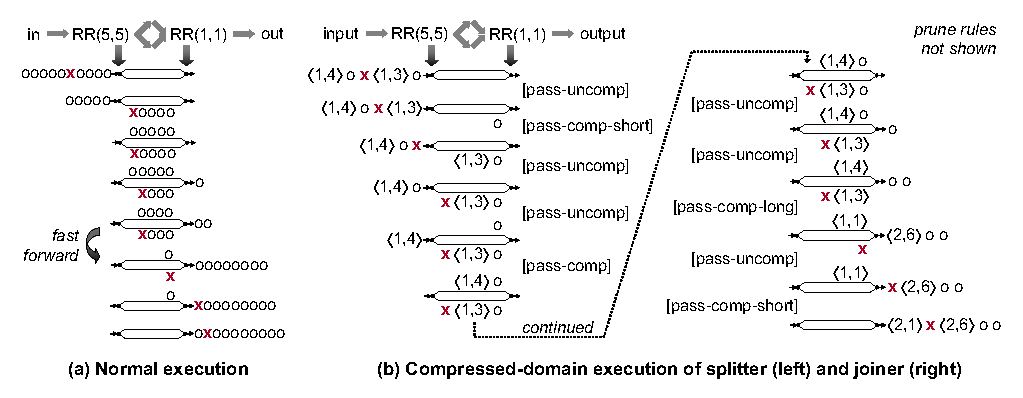
\psfig{file=compressed-splitjoin-example.eps,width=7in}
%% \vspace{6pt}
%% \caption{Example execution of splitters and joiners in the compressed
%%   domain.  As illustrated by the input/output pairs in (a), the
%%   example performs a transpose of a 2x5 matrix.  When the matrix is
%%   linearized (as in (b) and (c)), the input stream traverses the
%%   elements row-wise while the output stream traverses column-wise.
%%   Due to redundancy in the matrix, this reordering can be done largely
%%   in the compressed domain.  \protect\label{fig:sj-example}}
%% \end{figure*}

%% NOTE: the second point made in this section is not quite true,
%% since you still need to decompress RLE units that are a frame away
%% in Apple Animation.  Also first point seems redundant with align
%% being no-op for pop=1, so not including this.
%%
%% \subsubsection{Optimizations}
%% \label{sec:opt}
%%
%% As the transformation to the compressed domain is formulated in
%% fully general terms, the process can be streamlined considerably for
%% common classes of inputs:
%% \begin{itemize}
%% \item If a filter has a pop rate of one ($n=1$) on a given stream then
%%   no alignment stage is needed.
%% \item If the repeat distance is equal to the LZ77 window size, then no
%%   decompression is needed because it would simply overwrite the same
%%   values in the buffer.  This property holds for inter-frame repeats
%%   in the Apple Animation format (see Section~\ref{sec:formats}).
%% \end{itemize}
%% A consequence of the first bullet is that filters with a pop rate of
%% one (such as the InvertColor filter in Figure~\ref{fig:streamit}) avoid
%% performing any decompression, as there is no alignment stage.  This
%% guarantees that the output of the filter will be the same size as the
%% compressed input.

%% \subsection{Extensions}
%% \label{sec:extensions}

%% The transformation can be extended to support a broader class of
%% filters.  Some straightforward extensions are as follows:
%% \begin{itemize}

%% \item {\it Filters with state.}  If a filter retains mutable state from
%% one execution to the next, a repeat token can be copied across the
%% filter if the current state values are the same as they were at the
%% beginning of the repeated segment.  One could maintain a lookup table
%% that tracks the state values for the sake of this comparison.  Also,
%% state updates that have a closed form can be applied in the compressed
%% domain even if the current state has never been seen before; for
%% example, if a histogram filter runs for $n$ iterations on a blue
%% pixel, it will increment the blue count by $n$ regardless of the
%% initial value.

%% \item {\it Dynamic input and output rates.}  The current formulation
%% relies on a filter's fixed I/O rates to calculate repeat distances and
%% counts for the output tape from the repeat tokens on the input tapes.
%% However, in the presence of unpredictable I/O rates (e.g., edge
%% detection), a lookup table could be used to track the actual I/O rates
%% on each execution.  In the event of a repeat, the recorded I/O rates
%% from the previous execution could be used to calculate the repeat
%% parameters on the output tape.

%% \item {\it Sliding window computations.}  We currently assume that an
%% filter consumes all of the items it inspects on a given execution step.
%% However, some filters (e.g., a Gaussian blur filter) inspect a window
%% of values in addition to the one that is consumed.  Such {\it peeking}
%% filters can be supported by adjusting the translation of repeat
%% tokens, shortening the output count to match the period that the
%% entire window was within the repeated range.

%% \end{itemize}

%% \subsection{Splitters}

%% It is necessary to consider splitters and joiners separately from
%% general-purpose actors because of their pass-through semantics: the
%% inputs are distributed to the outputs without performing any
%% computation.  Our translation to the compressed domain leverages this
%% fact to preserve considerably more compression than would be possible
%% if splitters and joiners were viewed as opaque computational nodes
%% with multiple inputs and multiple outputs.  Consequently, splitters
%% and joiners should be employed by the programmer not only as a natural
%% expression of parallelism, but as a powerful way of exposing the data
%% reordering to the compiler.

%% As mentioned previously, splitters and joiners adopt a fine-grained
%% cyclo-static execution model, in which each execution step transfers
%% only one item from an input tape to an output tape.  That is, a
%% roundrobin$(k_1, k_2)$ splitter or joiner has $k_1 + k_2$ distinct
%% execution steps.  We refer to every group of $k_1 + k_2$ steps as an
%% {\it execution cycle}.

%% Duplicate splitters are trivial to transform to the compressed domain,
%% as all input tokens (both values and repeats) are copied directly to
%% the output streams.  For roundrobin splitters, the central concern is
%% that a repeat token can only be transferred to a given output tape if
%% the items referenced are also on that tape.  If the items referenced
%% by the repeat token were distributed to another tape, then the repeat
%% must be decompressed.

%% \begin{figure}[t]
%% \vspace{-1pt} % makes a page break difference, amazing
%% ~~~~~~~~~\psfig{figure=sj-figure.eps,width=2.8in}

%% \mbox{~~~~~~~~~~}(a) Notation for splitters~~~~~~~~~~~~~~(b) Notation for joiners
%% \caption{Notations used in the semantics for splitters and joiners.
%%   In addition, the variable $\pos$ indicates how many items have been
%%   written to (in the case of splitters) or read from (in the case of
%%   joiners) the active tape during the current execution cycle.
%%   \protect\label{fig:sj-pic}}
%% \end{figure}

%% The rest of this section focuses on roundrobin splitters.  To simplify
%% the presentation, we consider a splitter with only two output streams.
%% This captures all of the fundamental ideas; extension to additional
%% streams is straightforward.  Rewrite rules now take the following
%% form:

%% \hspace{-12pt}\begin{tabular}{l} ~ \vspace{-6pt} \\ 
%% \hspace{-3pt}$S \rightarrow T_1; T_2$ \hspace{-7pt}~\vspace{0.5pt} \\ \hline ~ \vspace{-7.5pt} \\
%% \hspace{-3pt}$S' \rightarrow T_1'; T_2'$ \hspace{-7pt} \\ ~ \vspace{-6pt} \\
%% \end{tabular}

%% \noindent where $T_1$ and $T_2$ represent the output streams of the
%% splitter (see Figure~\ref{fig:sj-pic}).  In addition, we make two
%% further simplifications:
%% \begin{itemize}

%% \item The rules assume that the next execution step of the splitter
%%   will write to $T_1$.  The subscripts should be interpreted without
%%   loss of generality.

%% \item We use $\pos$ to denote the number of items (in terms of the
%%   uncompressed domain) that have already been written to the current
%%   output stream ($T_1$) in the current execution cycle.  For brevity,
%%   the rules do not maintain the value of $\pos$, though it is
%%   straightforward to do so.

%% \end{itemize}

%% The semantics for splitter execution in the uncompressed domain appear
%% in Figure~\ref{fig:uncompressed-splitter}.  The {\tt
%%   pass-uncompressed} rule simply passes a single value from the input
%% tape to the current output tape, $T_1$.  Note that the current
%% position $\pos$ is implicitly incremented; once $\pos$ reaches $m_1$,
%% it is reset to zero and the output tapes are switched (tape $T_2$ will
%% be named $T_1$ on the next execution).

%% The compressed-domain semantics for splitters are given in
%% Figure~\ref{fig:compressed-splitter}, and a detailed example appears
%% in Figure~\ref{fig:sj-example}.  As mentioned previously, a repeat
%% token can be transferred to an output tape so long as the items
%% referenced also appear on that tape.  However, the repeat may need to
%% be fragmented (into several repeats of a lesser count), depending on
%% the repeat distance.  There are two cases to consider.

%% \begin{figure}[t]
%% $S \concat V \rightarrow T_1; T_2~~~~|V|=1$\name{pass-uncompressed}\skiptopb
%% ---------------------------------\skipbot
%% $S \rightarrow V \concat T_1; T_2$
%% \caption{Semantics of \textsc{Splitter}: execution of a roundrobin
%%   splitter in the uncompressed domain.
%%  \protect\label{fig:uncompressed-splitter}}
%% \end{figure}

%% \begin{figure}[t]
%% $S \concat V \rightarrow T_1; T_2~~~~|V|=1$\name{pass-uncompressed}\skiptopb
%% ---------------------------------\skipbot
%% $S \rightarrow V \concat T_1; T_2$
%% ~ \\ ~ \\
%% let~$\mbox{offset} = d$\%$(m_1+m_2)$\name{pass-compressed-long}\skiptopb
%% let~$(L_1, L_2) = \mbox{run\_splitter}(c)$\vspace{2pt}\\
%% $S \concat \tup{d}{c} \rightarrow T_1; T_2~~~~\mbox{offset} = 0$\vspace{-3pt}\skiptopa
%% --------------------------------------------\skipbot
%% $S \rightarrow \tup{d{\x}m_1/(m_1+m_2)}{L_1} \concat T_1;$\\
%% \mbox{~~~~~~~~~}\hspace{0.29pt}$\tup{d{\x}m_2/(m_1+m_2)}{L_2} \concat T_2$
%% ~ \\ ~ \\
%% let~$\mbox{offset} = d$\%$(m_1+m_2)$\name{pass-compressed-short}\skiptopb
%% let~$\mbox{offset'} = \mbox{\bf if~} \mbox{offset} \leq \pos \mbox{\bf ~then~} \mbox{offset}$\\
%% \mbox{~}\hspace{42.3pt}$\mbox{\bf ~else~} \mbox{offset} - m_2$\\
%% let~$\mbox{actual\_repeat} = \mbox{min}(c, \mbox{split\_potential}(d))$\\
%% $S \concat \tup{d}{c} \rightarrow T_1; T_2~~~~\mbox{offset} > 0~~~~\mbox{split\_potential}(d) > 0$\skiptopb
%% -------------------------------------------------------------------------\skipbot
%% $S \concat \tup{d}{c - \mbox{actual\_repeat}} \rightarrow$\\
%% $\tup{m_1*\mbox{floor}(d / (m_1 + m_2)) + \mbox{offset'}}{\mbox{actual\_repeat}} \concat T_1; T_2$
%% ~ \\ ~ \\
%% let~$\mbox{offset} = d$\%$(m_1+m_2)$\name{expand}\skiptopb
%% $S \concat \tup{d}{c} \rightarrow T_1; T_2~~\hspace{1pt}\mbox{offset} > 0~~\hspace{1pt}\mbox{split\_potential}(d) = 0$\skiptopb
%% -------------------------------------------------------------------\skipbot
%% $S \concat \tup{d}{c-1} \concat \mbox{\it decode}(\tup{d}{1}) \rightarrow T_1; T_2$
%% ~ \\ ~ \\
%% $S \concat \tup{d}{0} \rightarrow T_1; T_2$\name{prune}\skiptopb
%% ------------------------\skipbot
%% $S \rightarrow T_1; T_2$
%% \caption{Semantics of \textsc{Compressed-Splitter}:  execution of a roundrobin
%% splitter in the compressed domain.
%% \protect\label{fig:compressed-splitter}}
%% \end{figure}

%% % improve this explanation
%% The first case, expressed by the {\tt pass-compressed-long} rule in
%% Figure~\ref{fig:compressed-splitter}, distributes an entire repeat
%% token to both output tapes without any fragmentation.  This is only
%% possible when the repeat can be cleanly separated into two independent
%% sequences, one offset by $m_1$ and the next offset by $m_2$.  In other
%% words, the repeat distance must be a multiple of $m_1+m_2$.  In this
%% case, the repeat token is moved to the output streams.  The repeat
%% distance is scaled down to match the weight of each stream, and the
%% count is divided according to the current position of the splitter (a
%% simple but tedious calculation implemented by {\tt run\_splitter} in
%% Figure~\ref{fig:helper-splitter}).

%% \begin{figure}[t]
%% \begin{minipage}{0.1in}
%% \vspace{-1.75pt}
%% {\it // // // // //}
%% \end{minipage}
%% \begin{minipage}{3.23in}
%% {\it Given that $c$ items are available on input stream of a splitter,
%%   returns the number of items that can be written to each output stream
%%   before the input is exhausted.
%%   Assumes that the splitter is currently writing to the first output
%%   stream, to which \mbox{pos} items have previously been written in
%%   the current execution cycle.}
%% \end{minipage}
%% \mbox{\bf run\_splitter}$(c, \pos )$~returns~(int,~int)~\{\\
%% \tab{\it // the number of complete splitter cycles, and the leftover}\\
%% \tab$\mbox{total\_cycles} = \mbox{floor}(c/(m_1 + m_2))$\\
%% \tab$\mbox{total\_leftover} = c$\%$(m_1 + m_2)$\\
%% ~ \vspace{-6pt}\\ 
%% \tab{\it // the last partial cycle may end in three regions:}\\
%% \tab$\mbox{\bf if~} \mbox{total\_leftover} \leq m_1 - \pos$~\{\\
%% \tab\tab{\it // 1. in writing to the first output stream}\\
%% \tab\tab$L_1 = \mbox{total\_leftover}$\\
%% \tab\tab$L_2 = 0$\\
%% \tab$\} \mbox{\bf~else if~} \mbox{total\_leftover} \leq m_1-\pos + m_2~\{$\\
%% \tab\tab{\it // 2. in subsequent writing to the second output stream}\\
%% \tab\tab$L_1 = m_1-\pos$\\
%% \tab\tab$L_2 = \mbox{total\_leftover} - m_1-\pos$\\
%% \tab\} \mbox{\bf else} \{\\
%% \tab\tab{\it // 3. in wrap-around writing to the first output stream}\\
%% \tab\tab$L_1 = \mbox{total\_leftover} - m_2$\\
%% \tab\tab$L_2 = m_2$\\
%% \tab\}\\
%% ~ \vspace{-6pt}\\
%% \tab$\mbox{\bf return~}(m_1*\mbox{total\_cycles} + L_1, m_2*\mbox{total\_cycles} + L_2)$
%% \}\\
%% ~ \\
%% \begin{minipage}{0.1in}
%% \vspace{-1.75pt}
%% {\it // // // // //}
%% \end{minipage}
%% \begin{minipage}{3.23in}
%% {\it Given a repeat token with distance $d$ that is input to a
%%   splitter, returns the maximum count of a repeat token that could
%%   safely be emitted to the current output stream of the splitter.
%%   Assumes that only a single repeat token can be emitted (i.e., the
%%   {\tt pass-compressed-long} rule does not apply).}
%% \end{minipage}
%% \mbox{\bf split\_potential}$(d)$~returns~int~\{\\
%% \tab$\mbox{offset} = d$\%$(m_1 + m_2)$\\
%% \tab$\mbox{{\bf if~}} \mbox{offset} \leq \pos ~\{$\\
%% \tab\tab{\it // repeat for remainder of this execution cycle}\\
%% \tab\tab$\mbox{\bf return~} m_1 - \pos$\\
%% \tab$\} \mbox{\bf ~else if~} \mbox{offset} > m_2 + \pos ~\{$\\
%% \tab\tab{\it // repeat until referenced data goes out of range}\\
%% \tab\tab$\mbox{\bf return~} \mbox{offset} - (m_2 + \pos)$\\
%% \tab$\} \mbox{\bf ~else} ~\{$\\
%% \tab\tab{\it // referenced data is on the other output stream}\\
%% \tab\tab$\mbox{\bf return~} 0$\\
%% \tab$\}$\\
%% \}
%% \caption{Helper functions for \textsc{Compressed-Splitter}.
%% \protect\label{fig:helper-splitter}}
%% \end{figure}

%% The second case, handled by the {\tt pass-compressed-short} rule, is
%% when the repeat distance is mis-aligned with the splitter's execution
%% cycle, and thus the repeat (if it is long enough) eventually
%% references items that are distributed to a different output tape.
%% Nonetheless, part of the repeat may be eligible to pass through, so
%% long as the items referenced refer to the current output tape.  This
%% judgment is performed by {\tt split\_potential}
%% (Figure~\ref{fig:helper-splitter}) by comparing the repeat distance to
%% the current position in the output stream.  If one or more of the
%% repeated values are in range, the valid segment of the repeat (of
%% length {\tt actual\_repeat}) is moved to the output tape.  As before,
%% the repeat distance needs to be scaled according to the weights of the
%% splitter, and an extra offset is needed if the repeat distance wraps
%% around to reference the end of a previous cycle.

%% If neither of the above transfers apply, then the input stream needs
%% to be partially decompressed (according to the {\tt expand} rule)
%% because the current repeat token references items that will be sent to
%% the wrong output tape.  The {\tt prune} rule is also needed to clear
%% empty repeats generated by {\tt expand}.

%% Though we omit the details, it is also desirable to employ an analog
%% of the {\tt coarsen-repeat} rule (Figure~\ref{fig:stream-align}) to
%% preserve even more compression across a splitter.  The intuition is
%% that, by increasing certain repeat distances, the splitter's output
%% tapes can become more independent (referencing themselves rather than
%% each other).  This enables a compressed rule to fire in place of an
%% expansion step.

%% \subsection{Joiners}

%% Analogously to splitters, there are two ways to pass repeat tokens
%% through a joiner.  If the input streams contain compatible repeat
%% tokens, then they can be combined into a long repeat that spans
%% multiple execution cycles; otherwise, a shorter repeat is extracted
%% from only one of the streams.  Both of these cases are illustrated by
%% example in Figure~\ref{fig:sj-example}.  Unlike splitters, there is
%% never a need to decompress repeat tokens into values before passing
%% through a joiner.  Though the repeat length may shrink to one, it will
%% remain a reference to a previous item rather than becoming a value
%% itself.

%% In the uncompressed domain, joiners have the semantics given in
%% Figure~\ref{fig:uncompressed-joiner}.  The {\tt pass-uncompressed}
%% rule passes a single value from the current input tape ($S_1$) to the
%% output tape.  Analogously to splitters, the variable $\pos$ represents
%% the number of items that have been read from the current input tape
%% and is implicitly updated.  Once $\pos$ reaches $n_1$, it is reset to
%% zero and the input tapes are switched (tape $S_2$ will be named $S_1$
%% on the next execution).

%% The first and most powerful way to execute joiners in the compressed
%% domain is to combine repeat tokens from both input streams
%% %
%% \clearpage\noindent\clearpage\noindent % WTF - with just 1 it gets really weird!
%% %
%% (rule {\tt pass-compressed-long} in
%% Figure~\ref{fig:compressed-joiner}).  For this to be possible, both
%% repeat distances must be the same multiple of their respective joiner
%% weight ($n_1$ or $n_2$); the combined token has a repeat distance that
%% is a multiple of $n_1 + n_2$.  The {\tt run\_joiner} routine
%% (Figure~\ref{fig:helper-joiner}) calculates the maximum repeat length
%% depending on the current position of the joiner and the repeat lengths
%% of the inputs.

%% \begin{figure}[t]
%% $S_1 \concat V; S_2 \rightarrow T~~~~|V|=1$\name{pass-uncompressed}\skiptopb
%% ---------------------------------\skipbot
%% $S_1; S_2 \rightarrow V \concat T$
%% \caption{Semantics of \textsc{Joiner}: execution of a roundrobin
%%   joiner in the uncompressed domain.
%% \protect\label{fig:uncompressed-joiner}}
%% \end{figure}

%% \begin{figure}
%% $S_1 \concat V; S_2 \rightarrow T~~~~|V|=1$\name{pass-uncompressed}\skiptopb
%% ---------------------------------\skipbot
%% $S_1; S_2 \rightarrow V \concat T$
%% ~ \\ ~ \\
%% let~$(L_1, L_2) = \mbox{run\_joiner}(c_1, c_2, pos)$\name{pass-compressed-long}\skiptopb
%% $S_1 \concat \tup{d_1}{c_1};$\\
%% $S_2 \concat \tup{d_2}{c_2} \rightarrow T~~~~d_1$\%$n_1=0~~~~d_2$\%$n_2=0~~~~d_1/n_1=d_2/n_2$\vspace{-3pt}\skiptopa
%% --------------------------------------------------------------------------------\skipbot
%% $S_1 \concat \tup{d_1}{c_1-L_1};$\\
%% $S_2 \concat \tup{d_2}{c_2-L_2} \rightarrow \tup{d_1(n_1+n_2)/n_1}{L_1+L_2} \concat T$
%% ~ \\ ~ \\
%% let~$\mbox{offset'} = \mbox{\bf ~if~} d$\%$n_1 \leq \pos \mbox{\bf ~then~} \pos$\name{\hspace{-0.5pt}pass-compressed-short\hspace{1.5pt}(a)\hspace{-0.5pt}}\skiptopb
%% $\mbox{~~~~}\hspace{37.7pt}\mbox{\bf ~else~} d$\%$n_1 + n_2$\\
%% let~$L=\mbox{min}(c,\mbox{join\_potential}(d))$\\
%% $S_1 \concat \tup{d}{c}; S_2 \concat V \rightarrow T$\vspace{-3pt}\skiptopa
%% --------------------------------------------------\skipbot
%% $S_1 \concat \tup{d}{c-L}; S_2 \concat V \rightarrow$\\
%% $\tup{(n_1 + n_2){\x}\mbox{floor}(d/n_1) + \mbox{offset'}}{L} \concat T$
%% ~ \\ ~ \\
%% let~$\mbox{offset'} = \mbox{\bf ~if~} d$\%$n_1 \leq \pos \mbox{\bf ~then~} \pos$\name{\hspace{-0.7pt}pass-compressed-short\hspace{1.5pt}(b)\hspace{-0.7pt}}\skiptopb
%% $\mbox{~~~~}\hspace{37.7pt}\mbox{\bf ~else~} d$\%$n_1 + n_2$\\
%% let~$L=\mbox{min}(c,\mbox{join\_potential}(d))$\\
%% $S_1 \concat \tup{d}{c}; S_2 \concat \tup{d_2}{c_2} \rightarrow T~~~~d_2$\%$n_2 > 0$\vspace{-3pt}\skiptopa
%% -------------------------------------------------------\skipbot
%% $S_1 \concat \tup{d}{c-L}; S_2 \concat \tup{d_2}{c_2} \rightarrow$\\
%% $\tup{(n_1 + n_2){\x}\mbox{floor}(d/n_1) + \mbox{offset'}}{L} \concat T$
%% \\ ~ \\
%% $S_1 \concat \tup{d}{0}; S_2 \rightarrow T$\name{prune}\skiptopb
%% ------------------------\skipbot
%% $S_1; S_2 \rightarrow T$
%% \caption{Semantics of \textsc{Compressed-Joiner}.
%% \protect\label{fig:compressed-joiner}}
%% \end{figure}

%% \begin{figure}[t]
%% \begin{minipage}{0.1in}
%% \vspace{-1.75pt}
%% {\it // // // // // //}
%% \end{minipage}
%% \begin{minipage}{3.23in}
%% {\it Given that $c_1$ and $c_2$ items are available on the first and
%%   second input streams of a joiner, returns the number of items that
%%   can be read from each input before one of them is exhausted.
%%   Assumes that the joiner is currently reading from the first input
%%   stream, from which \mbox{pos} items have previously been consumed in
%%   the current execution cycle.}
%% \end{minipage}
%% \mbox{\bf run\_joiner}$(c_1, c_2, \pos )$~returns~(int,~int)~\{\\
%% \tab{\it // the number of complete joiner cycles, and the leftovers}\\
%% \tab$\mbox{total\_cycles} = \mbox{floor}(c/(n_1 + n_2))$\\
%% \tab$\mbox{leftover}_1 = c_1 - \mbox{total\_cycles} * n_1$\\
%% \tab$\mbox{leftover}_2 = c_2 - \mbox{total\_cycles} * n_2$\\
%% ~ \vspace{-6pt}\\
%% \tab{\it // the last partial cycle may end in three regions:}\\
%% \tab$\mbox{\bf if~} \mbox{leftover}_1 \leq n_1 - \pos$~\{\\
%% \tab\tab{\it // 1. in reading from the first input stream}\\
%% \tab\tab$L_1 = \mbox{leftover}_1$\\
%% \tab\tab$L_2 = 0$\\
%% \tab$\} \mbox{\bf~else if~} \mbox{leftover}_2 \leq n_2~\{$\\
%% \tab\tab{\it // 2. in subsequent reading from the second input stream}\\
%% \tab\tab$L_1 = n_1-\pos$\\
%% \tab\tab$L_2 = \mbox{leftover}_2$\\
%% \tab\} \mbox{\bf ~else} \{\\
%% \tab\tab{\it // 3. in wrap-around reading from the first input stream}\\
%% \tab\tab$L_1 = \mbox{leftover}_1$\\
%% \tab\tab$L_2 = n_2$\\
%% \tab\}\\
%% ~ \vspace{-6pt}\\ 
%% \tab$\mbox{\bf return~}(n_1*\mbox{total\_cycles} + L_1, n_2*\mbox{total\_cycles} + L_2)$
%% \}\\
%% ~ \\
%% \begin{minipage}{0.1in}
%% \vspace{-1.75pt}
%% {\it // // // // //}
%% \end{minipage}
%% \begin{minipage}{3.23in}
%% {\it Given a repeat token with distance $d$ on the current input
%%   stream of a joiner, returns the maximum count of a repeat token that
%%   could safely be emitted to the output stream.  Assumes that only a
%%   single repeat token is available (i.e., the {\tt
%%     pass-compressed-long} rule does not apply).}
%% \end{minipage}
%% \mbox{\bf join\_potential}$(d)$~returns~int~\{\\
%% \tab$\mbox{offset} = d$\%$n_1$\\
%% \tab$\mbox{{\bf if~}} \mbox{offset} \leq \pos ~\{$\\
%% \tab\tab{\it // repeat for remainder of this execution cycle}\\
%% \tab\tab$\mbox{\bf return~} n_1 - \pos$\\
%% \tab$\} \mbox{\bf ~else} ~\{$\\
%% \tab\tab{\it // repeat until referenced data goes out of range}\\
%% \tab\tab$\mbox{\bf return~} \mbox{offset} - \pos$\\
%% \tab$\}$\\
%% \}
%% \caption{Helper functions for \textsc{Compressed-Joiner}.
%% \protect\label{fig:helper-joiner}}
%% \end{figure}

%% The second mode of compressed joiner execution inputs only a single
%% repeat token, extracting the maximum length that can safely move to
%% the output.  This rule is needed when the previous one does not apply:
%% if the second stream ends in a value rather than a repeat ({\tt
%%   pass-compressed-short (a)}) or the repeat distance has the wrong
%% granularity ({\tt pass-compressed-short (b)}).  The {\tt
%%   join\_potential} routine (Figure~\ref{fig:helper-joiner}) determines
%% how much of the repeat can be moved to the output before the data
%% referenced would have originated from a different input stream.

%% As in the case of splitters, further compression gains are possible by
%% adding rules to coarsen the repeat distance or shift the distance to
%% align with other streams.  We omit the details here.
